\documentclass[10pt,a4paper,oneside]{book}
\usepackage[utf8x]{inputenc}
\RequirePackage[brazil,brazilian]{babel}
\usepackage{graphicx}
\usepackage{hyperref} %produz referncia clicveis no documento.
%\usepackage{subfigure}
\usepackage{graphicx}
%\usepackage{listings}
\usepackage{hyperref}
\usepackage[alf]{abntcite}
\usepackage{ae}
\usepackage{url}
\usepackage{caption}
\usepackage{vmargin}
\setmarginsrb{2cm}{1cm}{1.5cm}{1.5cm}{1cm}{0mm}{1.5cm}{0.5cm}

\usepackage{fancyhdr}
\pagestyle{fancy}
\fancyfoot[CO,CE]{Arduino}
\fancyfoot[RO, LE] {\thepage}
\fancyfoot[LO,LE]{EdutechKits}

\usepackage{listings}
\usepackage{color}
\usepackage{textcomp}
\definecolor{listinggray}{gray}{0.98}
\definecolor{lbcolor}{rgb}{0.98,0.98,0.98}
\lstset{
	backgroundcolor=\color{lbcolor},
	tabsize=4,
	rulecolor=,
	language=matlab,
        basicstyle=\scriptsize,
        upquote=true,
        aboveskip={1.5\baselineskip},
        columns=fixed,
        showstringspaces=false,
        extendedchars=true,
        breaklines=true,
        prebreak = \raisebox{0ex}[0ex][0ex]{\ensuremath{\hookleftarrow}},
        frame=single,
        showtabs=false,
        showspaces=false,
        showstringspaces=false,
        identifierstyle=\ttfamily,
        keywordstyle=\color[rgb]{0,0,1},
        commentstyle=\color[rgb]{0.133,0.545,0.133},
        stringstyle=\color[rgb]{0.627,0.126,0.941},
}

\author{Fernando Michelotti}
\title{Arduino}
\begin{document}

\maketitle
\tableofcontents
\listoffigures
\listoftables

\chapter{Introdução}

Iniciado como tradução de \cite{ItpPhysicalComputing}

Utilizando arduino \cite{SiteArduino}

Utilizando wiring \cite{SiteWiring}

\chapter{Arduino}

%http://www.arduino.cc/

Arduino is an open-source electronics prototyping platform based on flexible, easy-to-use hardware and software. It's intended for artists, designers, hobbyists, and anyone interested in creating interactive objects or environments.

\begin{figure}[!htb]
     \centering
     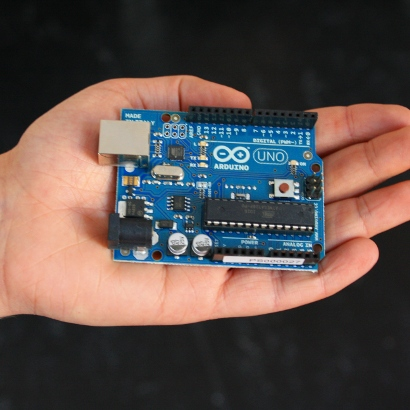
\includegraphics[scale=0.5]{img/arduino/arduino_uno_test.jpg}
     \caption{Arduino}
     \label{Arduino}
\end{figure}

Arduino can sense the environment by receiving input from a variety of sensors and can affect its surroundings by controlling lights, motors, and other actuators. The microcontroller on the board is programmed using the Arduino programming language (based on Wiring) and the Arduino development environment (based on Processing). Arduino projects can be stand-alone or they can communicate with software on running on a computer (e.g. Flash, Processing, MaxMSP).

The boards can be built by hand or purchased preassembled; the software can be downloaded for free. The hardware reference designs (CAD files) are available under an open-source license, you are free to adapt them to your needs.

Arduino received an Honorary Mention in the Digital Communities section of the 2006 Ars Electronica Prix. The Arduino team is: Massimo Banzi, David Cuartielles, Tom Igoe, Gianluca Martino, and David Mellis. Credits


\section{Programação para micro controladores}

\section{Arduino}

% WIKIPEDIA

Arduino is an open-source electronics prototyping platform, designed to make the process of using electronics in multidisciplinary projects more accessible. The hardware consists of a simple open hardware design for the Arduino board with an Atmel AVR processor and on-board I/O support. The software consists of a standard programming language and the boot loader that runs on the board.

Arduino hardware is programmed using a Wiring-based language (syntax + libraries), similar to C++ with some simplifications and modifications, and a Processing-based IDE.[1]

Currently shipping versions can be purchased pre-assembled; hardware design information is available for those who would like to assemble an Arduino by hand. Additionally, variations of the Italian-made Arduino—with varying levels of compatibility—have been released by third parties.

The Arduino project received an honorary mention in the Digital Communities category at the 2006 Prix Ars Electronica.[2][3]

The project began in Ivrea, Italy in 2005 to make a device for controlling student-built interaction design projects less expensively than other prototyping systems available at the time. As of February 2010 more than 120,000 Arduino boards had been shipped.[4] Founders Massimo Banzi and David Cuartielles named the project after a local bar named Arduino.[5] The name is an Italian masculine first name, meaning "strong friend". The English pronunciation is "Hardwin", a namesake of Arduino of Ivrea

\section{Platform}

\subsection{Hardware}

An official Arduino Duemilanove (rev 2009b).

An Arduino board consists of an 8-bit Atmel AVR microcontroller with complementary components to facilitate programming and incorporation into other circuits. An important aspect of the Arduino is the standard way that connectors are exposed, allowing the CPU board to be connected to a variety of interchangeable add-on modules (known as shields). Official Arduinos have used the megaAVR series of chips, specifically the ATmega8, ATmega168, ATmega328, and ATmega1280. A handful of other processors have been used by Arduino compatibles. Most boards include a 5 volt linear regulator and a 16 MHz crystal oscillator (or ceramic resonator in some variants), although some designs such as the LilyPad run at 8 MHz and dispense with the onboard voltage regulator due to specific form-factor restrictions. An Arduino's microcontroller is also pre-programmed with a bootloader that simplifies uploading of programs to the on-chip flash memory, compared with other devices that typically need an external chip programmer.

At a conceptual level, when using the Arduino software stack, all boards are programmed over an RS-232 serial connection, but the way this is implemented varies by hardware version. Serial Arduino boards contain a simple inverter circuit to convert between RS-232-level and TTL-level signals. Current Arduino boards are programmed via USB, implemented using USB-to-serial adapter chips such as the FTDI FT232. Some variants, such as the Arduino Mini and the unofficial Boarduino, use a detachable USB-to-serial adapter board or cable, Bluetooth or other methods. (When used with traditional microcontroller tools instead of the Arduino IDE, standard AVR ISP programming is used.)

The Arduino board exposes most of the microcontroller's I/O pins for use by other circuits. The Diecimila, now superseded by the Duemilanove, for example, provides 14 digital I/O pins, six of which can produce PWM signals, and six analog inputs. These pins are on the top of the board, via female 0.1 inch headers. Several plug-in application "shields" are also commercially available.

The Arduino Nano, and Arduino-compatible Bare Bones Board and Boarduino boards provide male header pins on the underside of the board to be plugged into solderless breadboards.

Sortable table
Arduino	Processor	Flash
KiB	EEPROM
KiB	SRAM
KiB	Digital I/O
pins	...with
PWM	Analog input
pins	Dimensions
Diecimila	ATmega168	16	0.5	1	14	6	6	2.7"x2.1"
Duemilanove	ATmega328	32	1	2	14	6	6	2.7"x2.1"
Uno	ATmega328	32	1	2	14	6	6	2.7"x2.1"
Mega	ATmega1280	128	4	8	54	14	16	4"x2.1"
Fio	ATmega328P	32	1	2	14	6	8	1.1"x1.6"
Mega2560	ATmega2560	256	4	8	54	14	16	4"x2.1"

\subsection{Software}

The Arduino IDE is a cross-platform application written in Java, and is derived from the IDE for the Processing programming language and the Wiring project. It is designed to introduce programming to artists and other newcomers unfamiliar with software development. It includes a code editor with features such as syntax highlighting, brace matching, and automatic indentation, and is also capable of compiling and uploading programs to the board with a single click. There is typically no need to edit makefiles or run programs on the command line.

The Arduino IDE comes with a C/C++ library called "Wiring" (from the project of the same name), which makes many common input/output operations much easier. Arduino programs are written in C/C++, although users only need define two functions to make a runnable program:

setup() – a function run once at the start of a program that can initialize settings

loop() – a function called repeatedly until the board powers off

A typical first program for a microcontroller simply blinks a LED (light-emitting diode) on and off. In the Arduino environment, the user might write a program like this:

\begin{verbatim}
#define LED_PIN 13
 
void setup () {
    pinMode (LED_PIN, OUTPUT);     // enable pin 13 for digital output
}
 
void loop () {
    digitalWrite (LED_PIN, HIGH);  // turn on the LED
    delay (1000);                  // wait one second (1000 milliseconds)
    digitalWrite (LED_PIN, LOW);   // turn off the LED
    delay (1000);                  // wait one second
}
\end{verbatim}

[7]
The above code would not be seen by a standard C++ compiler as a valid program, so when the user clicks the "Upload to I/O board" button in the IDE, a copy of the code is written to a temporary file with an extra include header at the top and a very simple main() function at the bottom, to make it a valid C++ program.
The Arduino IDE uses the GNU toolchain and AVR Libc to compile programs, and uses avrdude to upload programs to the board.
Official hardware

The Arduino Mega2560, uses a surface-mounted ATmega2560, bringing the total memory to 256 kB. It also incorporates the new ATmega8U2 USB chipset.

\subsection{Open hardware and open source}

\subsection{Main article: Open source hardware}

The Arduino hardware reference designs are distributed under a Creative Commons Attribution Share-Alike 2.5 license and are available on the Arduino Web site. Layout and production files for some versions of the Arduino hardware are also available. The source code for the IDE and the on-board library are available and released under the GPLv2 license.[1]

\subsection{Accessory hardware}


\subsection{A prototyping shield, mounted on an Arduino}

Arduino and Arduino-compatible boards make use of shields, which are printed circuit boards that sit atop an Arduino, and plug into the normally supplied pin-headers. These are expansions to the base Arduino. There are many functions of shields, from motor controls, to breadboarding (prototyping).[1]

For example:

\begin{itemize}
\item Arduino Ethernet Shield
\item XBee Shield
\item TouchShield from Liquidware
\item Datalog Shield: RTC, SD card storage, temperature sensing, etc. From NuElectronics
\item USB Host Shield from Circuits@Home
\item Cosmo WiFi Connect from JT5
\item A list of Arduino-compatible shields is maintained at the Arduino Shield List website.
\end{itemize}




\chapter{Componentes}

% http://itp.nyu.edu/physcomp/Labs/Components
\section{Voltage Regulator}

Voltage regulators take a range of DC voltage and convert it to a constant voltage. For example, this regulator, a 7805 regulator, takes a range of 8 - 15 volts DC input and converts it to a constant 5-volt output.

Note the label on the regulator that reads "7805". Check the label on every component. This physical form factor, called the package, is used by many different components, and not all of them are voltage regulators. This is a TO-220 package.

The 7800 series regulators come in many different voltages. 7805 is a 5-volt regulator. 7809 is a 9-volt regulator. 7812 is a 12-volt regulator. All the regulators of this family have the same pin connections. In the image above, the left leg is connected to the input voltage. The middle leg is connected to ground. The right leg is the output voltage.

\href{http://www.national.com/ds.cgi/LM/LM341.pdf}{7805 datasheet}

\begin{figure}[!htb]
     \centering
     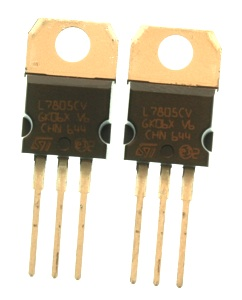
\includegraphics[scale=0.3]{img/components/v_reg_7805.jpg}
     \caption{5V voltage regulator}
     \label{5V voltage regulator}
\end{figure}

\begin{figure}[!htb]
     \centering
     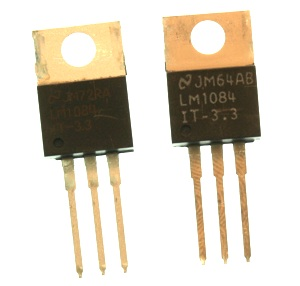
\includegraphics[scale=0.3]{img/components/v_reg_33v.jpg}
     \caption{3.3V voltage regulator}
     \label{3.3V voltage regulator}
\end{figure}

3.3V regulators are also common. Note that these ones don't have the same pin configuration as the 7805 regulators!

\section{LED}

\begin{figure}[!htb]
     \centering
     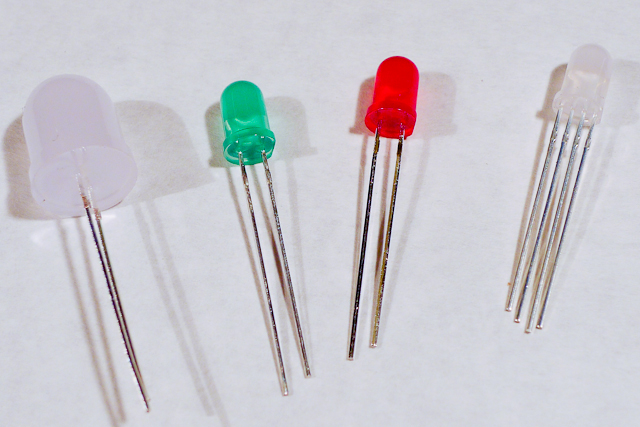
\includegraphics[scale=0.3]{img/components/leds.jpg}
     \caption{LEDs}
     \label{LEDs}
\end{figure}

LEDs, or Light Emitting Diodes, are diodes that emit light when given the correct voltage. Like all diodes, they are polarized, meaning that they only operate when oriented correctly in the circuit. The anode of the LED connects to voltage, and the cathode connects to ground. The anode in the LEDs in this photo is the longer leg on each LED. LEDs come in many diferent packages. The packages above have built-in lenses.
These LEDs are the cheapest you can buy, and they're not very bright. You can get superbright LEDs as well, which are much brighter. If you're working on applications that need very small light sources, you can also get LEDs in a surface mount package.
LEDs can only handle a limited amount of current and voltage. The details should be covered in each LED's datasheet, but if not, here's a link to a handy LED current calculator. For most common LEDs running at 5 volts, a resistor between 220 and 1K ohms will do the job.

\begin{figure}[!htb]
     \centering
     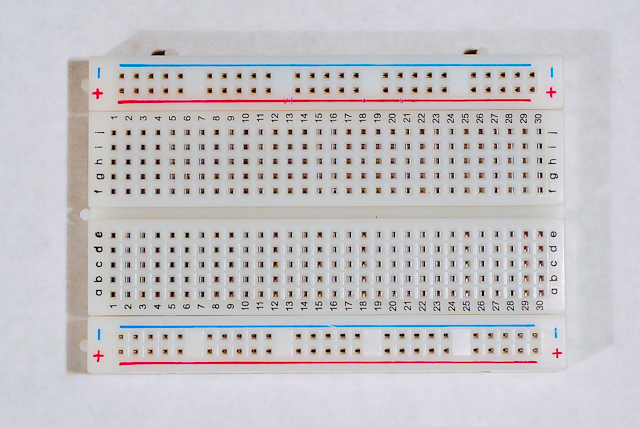
\includegraphics[scale=0.55]{img/components/breadboard_short.jpg}
     \caption{solderless breadboard}
     \label{solderless breadboard}
\end{figure}



\section{Resistors}

Resistors resist the flow of electrical current. When placed in series, they reduce the voltage, and limit the current. The bands on a resistor indicate the resistor's value. Here's a handy resistor color code calculator. 

\begin{figure}[!htb]
     \centering
     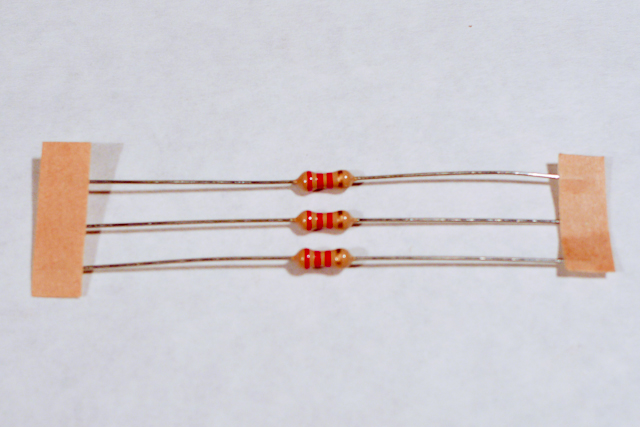
\includegraphics[scale=0.3]{img/components/resistors.jpg}
     \caption{resistors}
     \label{resistors}
\end{figure}

\section{Potentiometers}


Potentiometers are variable resistors. The two outside terminals act as a fixed resistor. A movable contact called the wiper moves across the resistor, producing a variable resistance between the center terminal and either of the two sides. 

\begin{figure}[!htb]
     \centering
     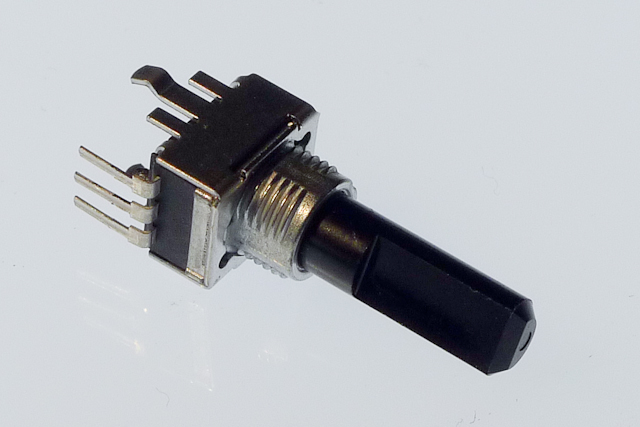
\includegraphics[scale=0.25]{img/components/potentiometer.jpg}
     \caption{potentiometer}
     \label{potentiometer}
\end{figure}

\subsection{trimmer potentiometers}
Trimmer potentiometers are designed to be mounted on a circuit board, difficult to turn, so you can use them to adjust a circuit. They're handy to use as physical variables, to tune your project. 

\begin{figure}[!htb]
     \centering
     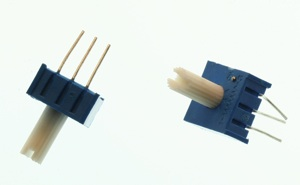
\includegraphics[scale=0.3]{img/components/pots_trimmer.jpg}
     \caption{trimmer potentiometer}
     \label{trimmer potentiometer}
\end{figure}

\section{Switches}

Switches are one form of digital input. There are many kinds of switches. The two most useful caategories are \textbf{momentary switches}, which remain closed only when you press them, and \textbf{toggle switches}, which stay in place after you switch them. 

\begin{figure}[!htb]
     \centering
     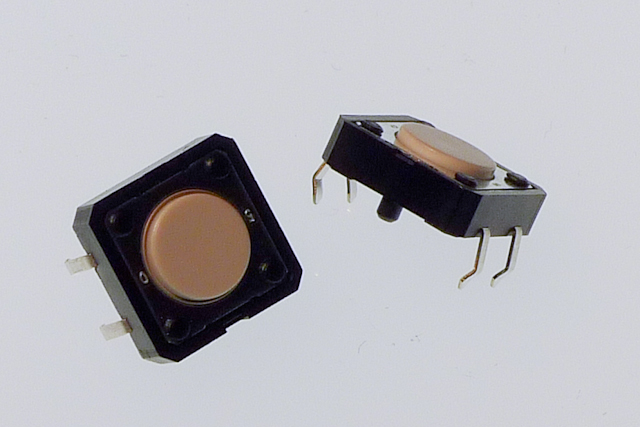
\includegraphics[scale=0.3]{img/components/switches_momentary.jpg}
     \caption{momentary switches}
     \label{momentary switches}
\end{figure}

\begin{figure}[!htb]
     \centering
     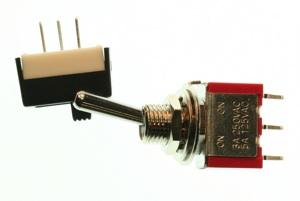
\includegraphics[scale=0.3]{img/components/switches_toggle.jpg}
     \caption{toggle switches}
     \label{toggle switches}
\end{figure}

\section{Photocells}

Photocells are variable resistors whose resistance changes as the light hitting them changes.

\begin{figure}[!htb]
     \centering
     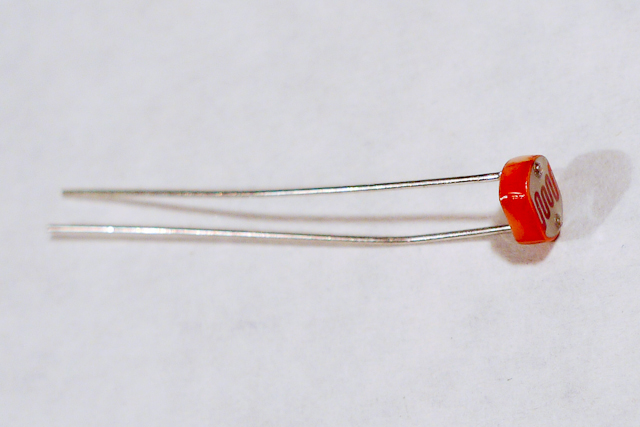
\includegraphics[scale=0.3]{img/components/photocell.jpg}
     \caption{photocell}
     \label{photocell}
\end{figure}

\section{Thermistors}

Thermistors are variable resistors whose resistance changes as the temperature changes. 

\begin{figure}[!htb]
     \centering
     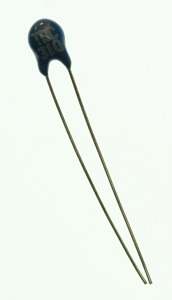
\includegraphics[scale=0.5]{img/components/thermistor.jpg}
     \caption{thermistor}
     \label{thermistor}
\end{figure}



\section{Capacitors}

Capacitors store electrical energy while there's energy coming in, and release it when the incoming energy stops. They have a variety of uses. One common use is to smooth out the dips and spikes in an electrical supply. This use is called decoupling.

\begin{figure}[!htb]
     \centering
     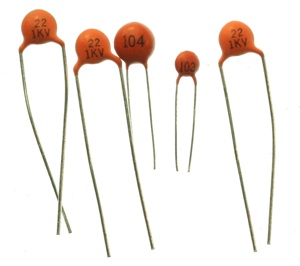
\includegraphics[scale=0.3]{img/components/caps_ceramic.jpg}
     \caption{ceramic capacitors}
     \label{ceramic capacitors}
\end{figure}

LEDs, or Light Emitting Diodes, are diodes that emit light when given the correct voltage. Like all diodes, they are polarized, meaning that they only operate when oriented correctly in the circuit. The anode of the LED connects to voltage, and the cathode connects to ground. The anode in the LEDs in this photo is the longer leg on each LED. LEDs come in many diferent packages. The packages above have built-in lenses.

\begin{figure}[!htb]
     \centering
     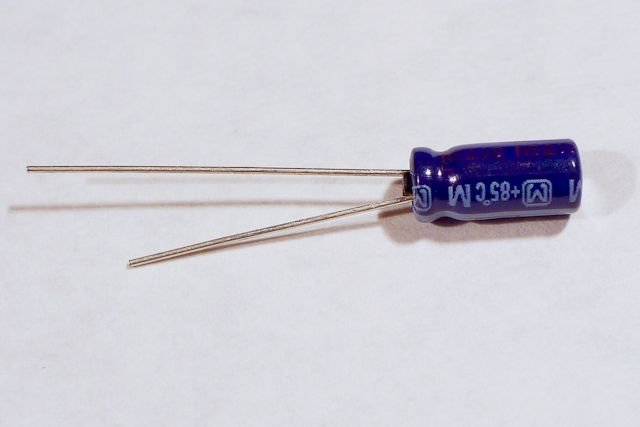
\includegraphics[scale=0.3]{img/components/caps_electrolytic.jpg}
     \caption{electrolytic capacitors}
     \label{electrolytic capacitors}
\end{figure}

Ceramic capacitors are cheap and unpolarized. They generally have very small capaacitance values. They're useful decoupling caps in a low-current circuit. You often see them used to decouple the power going into a microcontroller or other integrated circuit.
The number on a ceramic cap gives you its value and order of magnitude. For example, 104 indicates a 0.1 microfarad (uF) cap. 103 indicates a 0.001 microfarad cap. 

\begin{figure}[!htb]
     \centering
     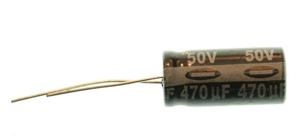
\includegraphics[scale=0.3]{img/components/cap_electrolytic_detail.jpg}
     \caption{electrolytic capacitor detail}
     \label{electrolytic capacitor detail}
\end{figure}


Electrolytic capacitors can generally store more charge than ceramic caps, and are longer lasting and more expensive. They're usually polarized, meaning that they have a positive leg and a negative leg. This is because current flows more efficiently through them one way than the other. 

An electrolytic cap will have a + or - on one side, as shown here. 

\section{Diodes}

\begin{figure}[!htb]
     \centering
     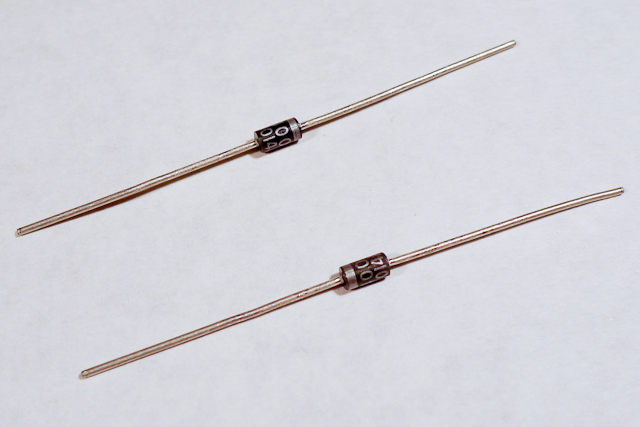
\includegraphics[scale=0.3]{img/components/diodes_400x.jpg}
     \caption{1N4001 diodes}
     \label{1N4001 diodes}
\end{figure}

Diodes permit voltage to flow in one direction and block it in the other direction. LEDs are a type of diode, as are the 1N4001 diodes shown here. They're useful for stopping voltage from going somewhere you don't want it to go. 

\begin{figure}[!htb]
     \centering
     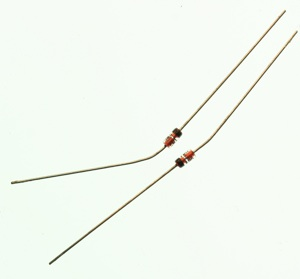
\includegraphics[scale=0.3]{img/components/diodes_zener.jpg}
     \caption{zener diodes}
     \label{zener diodes}
\end{figure}


Zener diodes have a breakdown voltage past which they allow current to flow in both directions. They're used to chop off excess voltage from a part of a circuit.

\section{Transistors}

\begin{figure}[!htb]
     \centering
     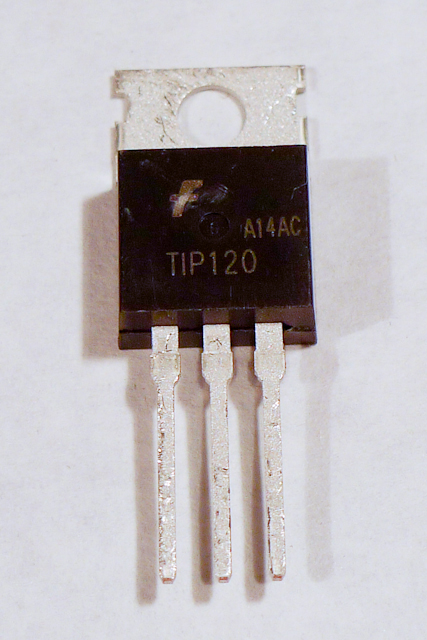
\includegraphics[scale=0.3]{img/components/transistors.jpg}
     \caption{transistors}
     \label{transistors}
\end{figure}

Transistors act as electronic switches. When you put a small voltage across the base and emitter, the transistor allows a larger current and voltage to flow from the collector to the emitter.

\section{Power Jacks}

\begin{figure}[!htb]
     \centering
     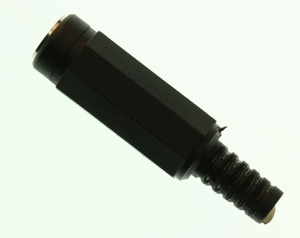
\includegraphics[scale=0.5]{img/components/power_jack.jpg}
     \caption{DC power jack, disassembled}
     \label{DC power jack, disassembled}
\end{figure}

\begin{figure}[!htb]
     \centering
     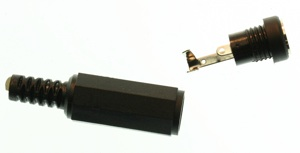
\includegraphics[scale=0.3]{img/components/power_jack_2.jpg}
     \caption{DC power jack}
     \label{DC power jack}
\end{figure}

\section{Battery Holders}

\begin{figure}[!htb]
     \centering
     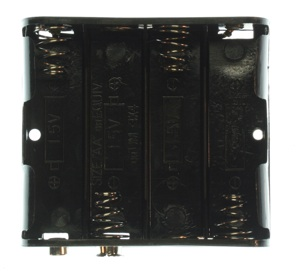
\includegraphics[scale=0.5]{img/components/battery_holder.jpg}
     \caption{AA battery holder}
     \label{AA battery holder}
\end{figure}


\begin{figure}[!htb]
     \centering
     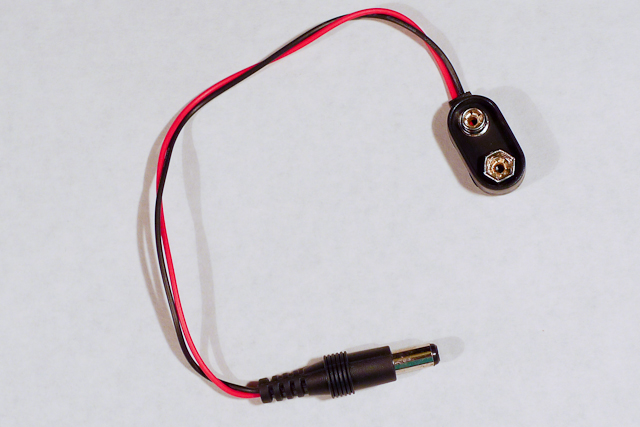
\includegraphics[scale=0.3]{img/components/battery_snap.jpg}
     \caption{9V battery snap}
     \label{9V battery snap}
\end{figure}

\section{Motors}

\subsection{Servo Motor}

\begin{figure}[!htb]
     \centering
     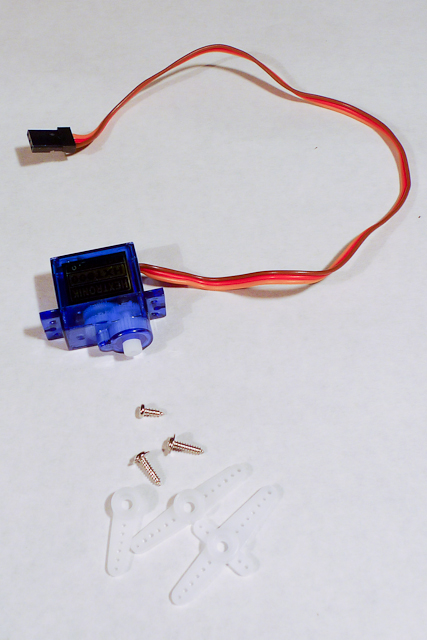
\includegraphics[scale=0.3]{img/components/servomotor.jpg}
     \caption{servomotor}
     \label{servomotor}
\end{figure}


\subsection{DC Motor}

\begin{figure}[!htb]
     \centering
     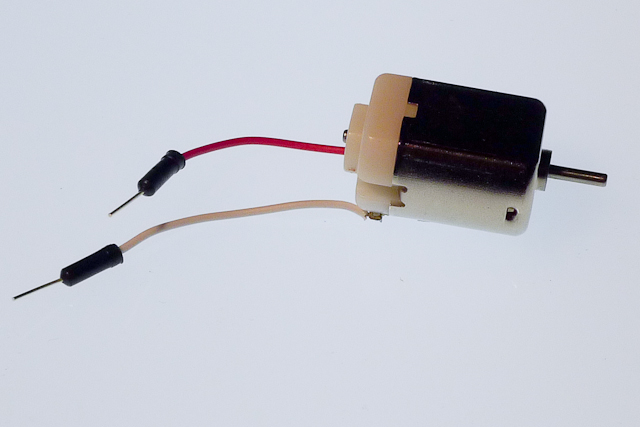
\includegraphics[scale=0.3]{img/components/dc_motor.jpg}
     \caption{DC motor}
     \label{DC motor}
\end{figure}


\section{Gear Kit}

\begin{figure}[!htb]
     \centering
     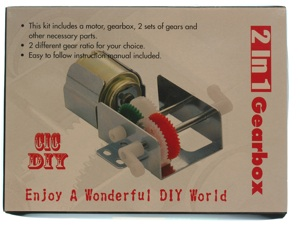
\includegraphics[scale=0.5]{img/components/gear_kit.jpg}
     \caption{gearbox kit}
     \label{LEDs}
\end{figure}


\section{H-Bridge}

\begin{figure}[!htb]
     \centering
     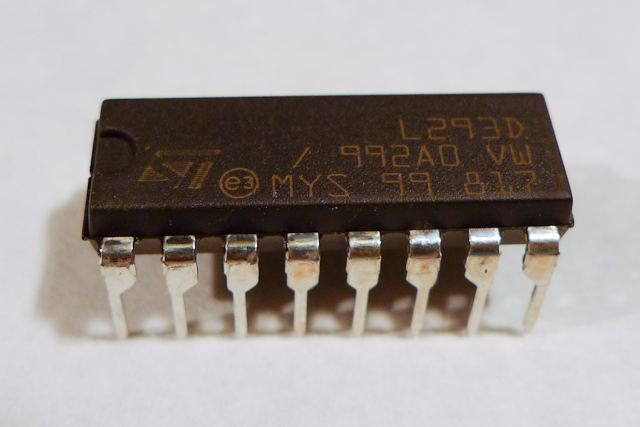
\includegraphics[scale=0.3]{img/components/h_bridge.jpg}
     \caption{H-bridge}
     \label{H-bridge}
\end{figure}


\section{Reed Relay}

\begin{figure}[!htb]
     \centering
     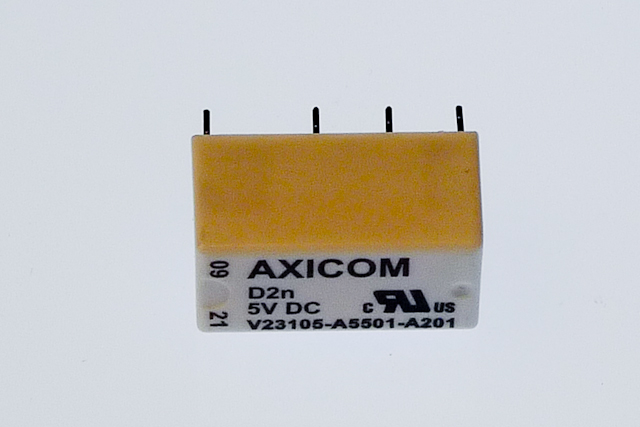
\includegraphics[scale=0.3]{img/components/relay.jpg}
     \caption{reed relay}
     \label{reed relay}
\end{figure}

\section{Screw Terminal}

\begin{figure}[!htb]
     \centering
     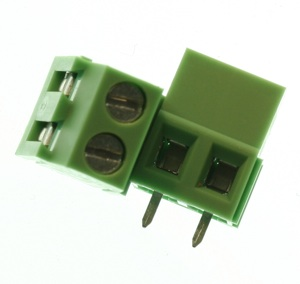
\includegraphics[scale=0.3]{img/components/screw_terminals.jpg}
     \caption{screw terminals}
     \label{screw terminals}
\end{figure}




\chapter{Set Up}


\chapter{Setting up a breadboard}

\begin{figure}[!htb]
     \centering
     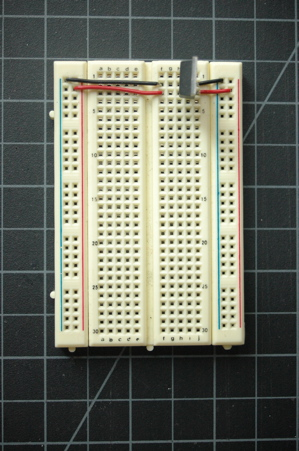
\includegraphics[scale=0.8]{img/breadboard/bboard_vreg_3.jpg}
     \caption{breadboard}
     \label{breadboard}
\end{figure}

Solderless beadboards are the quickest tools for prototyping a new circuit. For a detailed description of a breadboard, check these notes.

The picture at left shows a typical breadboard with a 7805 5-volt voltage regulator mounted on it. There are several rows of holes for components. The holes on the breadboard are separated by 0.1-inch spaces, and are organized in many short rows in the center, and in two long rows down each side of the board. The short horizontal rows in the middle are separated by a center divider. The pattern varies from model to model; some breadboards have only one strip down each side , others have multiple side rows, and some have no side rows.

On each side of the board are two long rows of holes, with a blue or a red line next to each row. All the holes in each of these lines are connected together with a strip of metal in the back. In the center are several short rows of holes separated by a central divider. All of the five holes in each row in the center are connected with a metal strip as well. This allows you to use the holes in any given row to connect components together. To see which holes are connected to which, take a multimeter and a couple of wires, set the multimeter to measure continuity, stick the two wires in two holes, and measure them with the multimeter. If the meter indicates continuity, then the two holes in question are connected.

\begin{figure}[!htb]
     \centering
     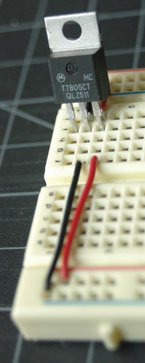
\includegraphics[scale=0.8]{img/breadboard/bboard_vreg_2.jpg}
     \caption{breadboard}
     \label{breadboard}
\end{figure}

The reason for the center divider is so that we can mount integrated circuit chips, like a microprocessor, on the breadboard. IC chips typically have two rows of pins that we need to connect other components to. The center row isolates the two rows from each other, and gives us several holes connected to each pin, so we can connect other components.

\textbf{When you start to put components on your breadboard, avoid adding, removing, or changing components on a breadboard whenever the board is powered. You risk shocking yourself and damaging your components.}

\begin{figure}[!htb]
     \centering
     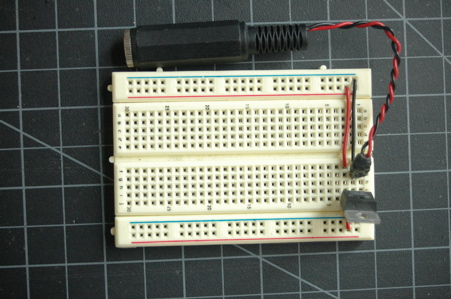
\includegraphics[scale=0.8]{img/breadboard/bboard_vreg_power_conn.jpg}
     \caption{breadboard}
     \label{breadboard}
\end{figure}

The regulator in the picture above is there to supply 5 volts to the two red side rows. The two blue side rows are connected to ground. These will be your power and ground bus rows. They give you lots of convenient places to connect to power or ground as needed. The red and black wires (red for power, black for ground) connect the bus rows to the rows where the regulator's ground and output pins are plugged in. The image at right shows a closeup on the connections to the regulator pins' rows.
With your board connected like this, you'll be able to build many different 5-volt circuits on the board. The last thing you need to add is a power connector to connect 8 - 12 volts DC to supply power for the voltage regulator. The image below shows a power connector connected to the input and ground pins of the voltage regulator.


\chapter{Soldering}

\section{Overview}

If you're going to do any electronics work, you're going to have to do some soldering. Many people fear it before they've done it, but it's really pretty simple to do. This exercise will show you how to solder a DC power connector to a set of wires for a breadboard.

\subsection{Parts}

To do it, you'll need:

\begin{figure}[!htb]
     \centering
     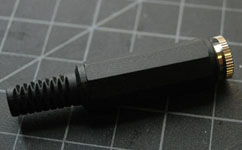
\includegraphics[scale=0.3]{img/soldering/power_connector.jpg}
     \caption{DC Power Jack}
     \label{DC Power Jack}
\end{figure}

\begin{figure}[!htb]
     \centering
     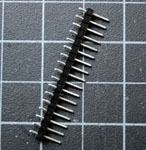
\includegraphics[scale=0.3]{img/soldering/headers.jpg}
     \caption{Header Pins}
     \label{Header Pins}
\end{figure}

\begin{figure}[!htb]
     \centering
     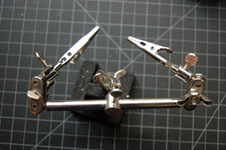
\includegraphics[scale=0.3]{img/soldering/helping_hands.jpg}
     \caption{Helping Hands}
     \label{Helping Hands}
\end{figure}

\begin{figure}[!htb]
     \centering
     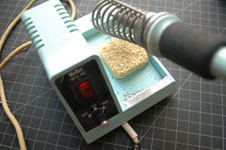
\includegraphics[scale=0.3]{img/soldering/soldering_iron.jpg}
     \caption{Soldering Iron}
     \label{Soldering Iron}
\end{figure}

\begin{figure}[!htb]
     \centering
     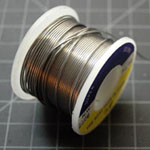
\includegraphics[scale=0.3]{img/soldering/solder.jpg}
     \caption{Solder}
     \label{Solder}
\end{figure}

\begin{figure}[!htb]
     \centering
     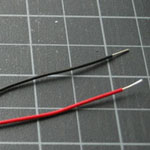
\includegraphics[scale=0.3]{img/soldering/hookup_wire.jpg}
     \caption{22-AWG hookup wire, in red and black}
     \label{22-AWG hookup wire, in red and black}
\end{figure}

\begin{figure}[!htb]
     \centering
     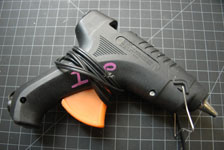
\includegraphics[scale=0.3]{img/soldering/hot_glue_gun.jpg}
     \caption{Hot Glue Gun and Hot Glue}
     \label{Hot Glue Gun and Hot Glue}
\end{figure}

\begin{figure}[!htb]
     \centering
     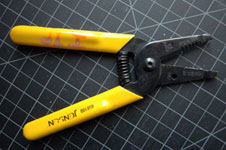
\includegraphics[scale=0.3]{img/soldering/wire_strippers.jpg}
     \caption{Wire Strippers}
     \label{Wire Strippers}
\end{figure}

\subsection{Preparing the parts}

Cut a red and a black wire about four inches in length. Strip the ends back about 1/4 of an inch. Bend a hook on one end of each wire. Unscrew the power jack. Connect the red wire to hole in the the center tab of the power, and the black to the hole in the outside tab. Use pliers to crimp the hooked wires to their connections on the jack. If the connections aren't soldered, you'll get an inconsistent connection at best, and a short circuit at worst.

\begin{figure}[!htb]
     \centering
     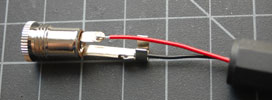
\includegraphics[scale=0.8]{img/soldering/power_connector_unsoldered.jpg}
     \caption{power connector unsoldered}
     \label{power connector unsoldered}
\end{figure}

\subsection{Soldering}

Touch the iron to the joint between the wire and the metal to heat the joint. Then touch the solder to the joint (NOT to the iron) until it melts. This should make a clean solder with a small blob of solder. Twist the wires together and thread them through the sleeve of the jack.

\begin{figure}[!htb]
     \centering
     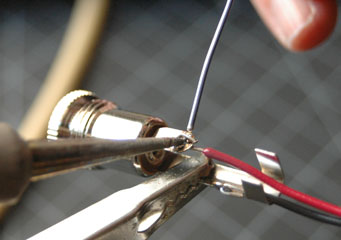
\includegraphics[scale=0.8]{img/soldering/soldering_power_connector.jpg}
     \caption{soldering power connector}
     \label{soldering power connector}
\end{figure}

The result should look like this:

\begin{figure}[!htb]
     \centering
     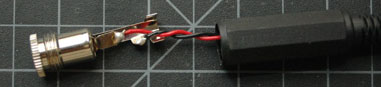
\includegraphics[scale=2.5]{img/soldering/power_conn_inside.jpg}
     \caption{power connector inside}
     \label{power connector inside}
\end{figure}


Trim the ends of the wires to the same length, and strip them back to about 1/8th of an inch. Break off two header pins and hold them in one clip of the helping hands. Clip the wires in the other clip, and align them with the header pins like so:

\begin{figure}[!htb]
     \centering
     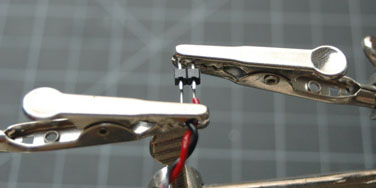
\includegraphics[scale=2.5]{img/soldering/soldering_headers.jpg}
     \caption{soldering headers}
     \label{LEDs}
\end{figure}

When you're done soldering, you should have two separate blobs like this:

\begin{figure}[!htb]
     \centering
     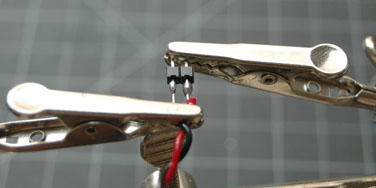
\includegraphics[scale=2.5]{img/soldering/soldering_headers_2.jpg}
     \caption{soldering headers 2}
     \label{soldering headers 2}
\end{figure}



If you can't see space between the two solder joints, de-solder them and do it again. You need to be sure there's no connection between these wires that can cause a short circuit, and the best way to do that is to leave space.
Take a hot glue gun and surround the bare connections to protect them and provide some strain relief. When you're done, you should have a connection like this:

\begin{figure}[!htb]
     \centering
     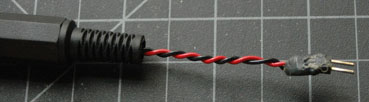
\includegraphics[scale=2.5]{img/soldering/power_conn_headers.jpg}
     \caption{power connector headers}
     \label{power connector headers}
\end{figure}

Make sure you can tell which pin is connected to the red wire and which is connected to the black.

\subsection{Testing}

Before you connect it to power, take a meter and check the connections for continuity. The center pin should be connected to the red wire, and the outer rim should be connected to black. When that's good, you're ready to use it.


\chapter{Introduction to electronics}


\chapter{Switches}

\section{Switch Terminology}

There are a few basic terms that get used with switches all the time.

Normally Open means that when the switch is in its normal position, the contacts are not touching, or open. Normally closed means that when the switch is in its normal position, the contacts are touching, or closed.

Single Throw means there's only two contacts. The switch is open or closed. Dual Throw means there's at least three contacts, and switching the switch moves the center contact from being closed with one outer contact to being closed with the other outer contact.

Single Throw means there's only one ser of contacts being closed or open by the switch's mechanism. Dual Throw means there's two sets of contacts being controlled by the same mechanism. With a dual throw switch, you can switch two separate circuits with the same mechanism.

\subsection{There are lots of types of switches.}

A few types are shown here:

\begin{figure}[!htb]
 \centering
 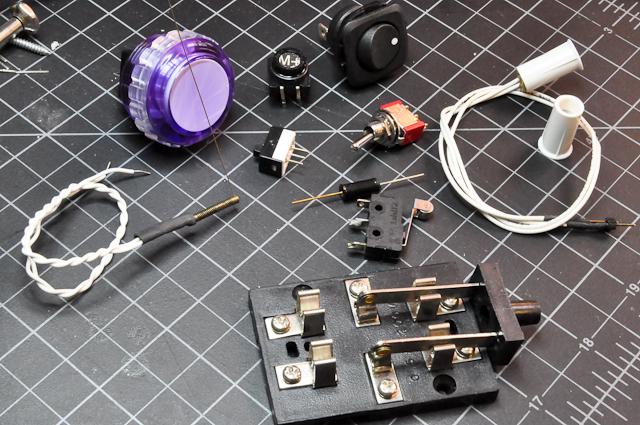
\includegraphics[scale=0.3]{img/switches/switches.jpg}
 \caption{various types of switches}
 \label{various types of switches}
\end{figure}

Pushbuttons or momentary switches stay closed only as long as you hold them closed. Roller switches are pushbuttons with a lever and a roller attached. They're useful when you need something to push against the switch gently to close it.

\begin{figure}[!htb]
 \centering
 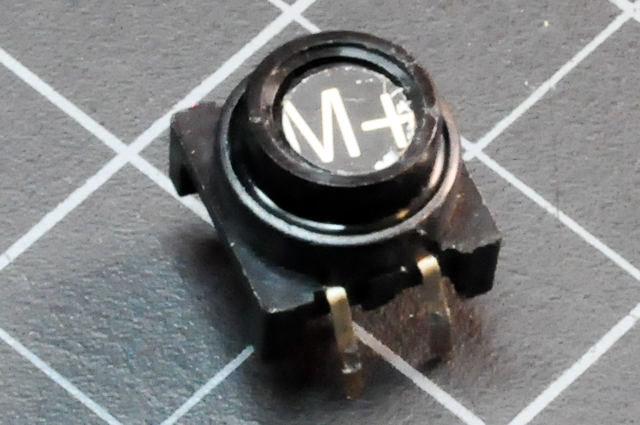
\includegraphics[scale=0.3]{img/switches/pushbutton.jpg}
 \caption{pushbutton}
 \label{pushbutton}
\end{figure}

\begin{figure}[!htb]
 \centering
 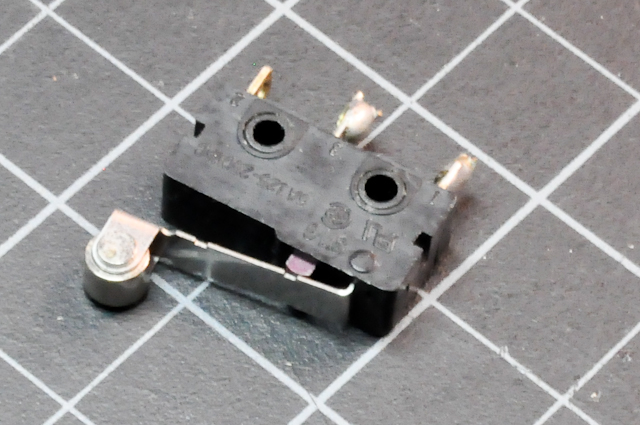
\includegraphics[scale=0.3]{img/switches/roller_switch.jpg}
 \caption{roller switch}
 \label{roller switch}
\end{figure}

Toggle switches stay closed in one physical position and open in the other. Slide switches are similar to toggle switches.

\begin{figure}[!htb]
 \centering
 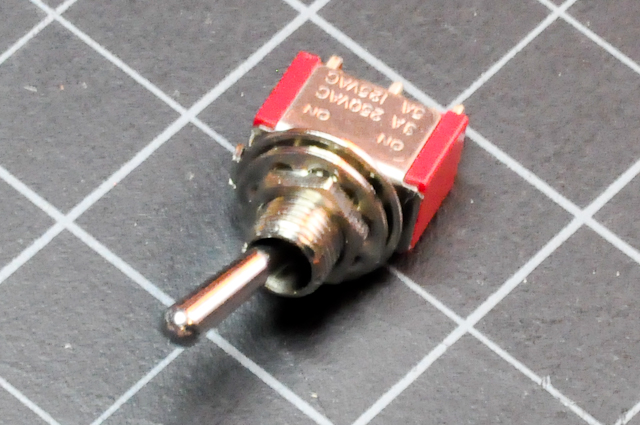
\includegraphics[scale=0.3]{img/switches/toggle_switch.jpg}
 \caption{toggle switch}
 \label{toggle switch}
\end{figure}

\begin{figure}[!htb]
 \centering
 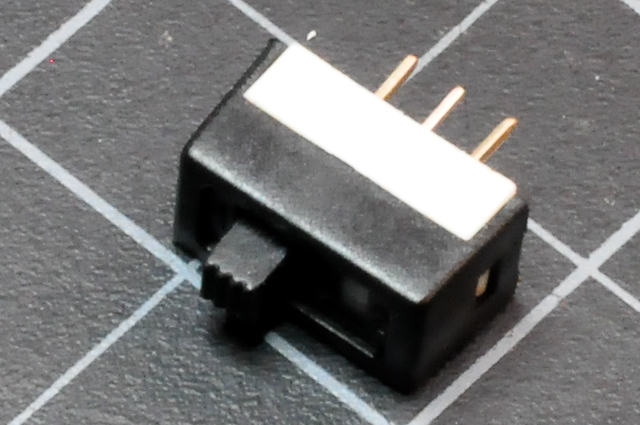
\includegraphics[scale=0.3]{img/switches/slide_switch.jpg}
 \caption{slide switch}
 \label{slide switch}
\end{figure}

Magnetic switches have two metal leaves in the end that are pulled together when a magnet is brought close to them. They're useful when you can't have wires on both sides of the switch mechanism.

\begin{figure}[!htb]
 \centering
 \includegraphics[scale=0.3]{img/switches/magnetic_snap.jpg}
 \caption{magnetic snap}
 \label{magnetic snap}
\end{figure}

Magnetic snaps are useful when you're making a soft circuit and need a fastener on the garment to close a switch.

Magnetic Snap

Whisker switches are made from a piece of spring steel or piano wire, and a center post. An insulator such as a piece of electrical tape or shrinkwrap holds the two separate. When the wire is touched, the spring bends and touches the metal post, and closes the switch. Solarbotics sells some nice whisker switches.

Whisker Switch

Tilt switches contain a metal ball and contacts at one end. When you tilt the switch, the ball touches both contacts, and closes the switch. There are also mercury switches that do the same, but with a ball of mercury inside. Avoid these, since mercury is very poisonous.

Whisker Switch

\section{Get Creative With Switches}

A switch is nothing more than a mechanism to bring two pieces of conductive material together and separate them. You can make a switch from any two conductors and a little creativity. Consider, for example:

conductive fabric

wire mesh

copper tape

All you need to do is arrange the two conductors in such a way that they can touch or not touch. Sometimes a spacer layered between the two conductors helps. For example, in this image you see three pieces of conductive fabric. Two of the pieces have non-conductive layers on top of them. When the non-conductive part is sandwiched between the conductive layers, you've got a switch that's pressed by touching. The conductive parts touch when they're pressed through the holes in the non-conductive part. These two switches would have different sensitivities because the hole-to-material ratio of the non-conductive layer is different.

soft switches

Make your own switch. Find a way to turn a closing door into a switch, for example, or to close a switch when a person sits down. Or figure out how to turn a hat into a switch, or a cane, or a zipper. Or perhaps the pieces of a puzzle can be switches.

Come up with an everyday activity to which you can add three or four custom switches that, when combined, turn on a light. For example, maybe the light comes on when you close the door, sit down, and open a book. Or when you walk upstairs, put your keys on a side table, and remove your hat. Combine your creativity with switches with what you learned in the electronics lab to make this happen.

For more ideas on materials, check out How to Get What You Want. They have an excellent list of conductive materials and instructions.

\section{Arrangements of switches}

In planning your switch project, consider what happens when you arrange switches in different ways. For example, try this circuit:

\subsection{Three switches in parallel. Any one of the three will turn on the LED}


Switches in parallel -- schematic

Switches in parallel -- breadboard

\subsection{Three switches in series. All three must be on to turn on the LED}


Switches in series -- schematic

Switches in series -- breadboard

Through a combination of series and parallel switches, you can come up with a variety of combinations that make the light turn on. Depending on where you add the LEDs, you can even have the same switches turn on different LEDs in different combinations. Try a few combinations and see what happens.

\begin{figure}[!htb]
 \centering
 \includegraphics[scale=0.3]{img/switches/conductive_fabric.jpg}
 \caption{conductive fabric}
 \label{conductive fabric}
\end{figure}


\begin{figure}[!htb]
 \centering
 \includegraphics[scale=0.3]{img/switches/copper_tape.jpg}
 \caption{copper tape}
 \label{copper tape}
\end{figure}





\begin{figure}[!htb]
 \centering
 \includegraphics[scale=0.3]{img/switches/magnetic_switch.jpg}
 \caption{magnetic switch}
 \label{magnetic switch}
\end{figure}











\begin{figure}[!htb]
 \centering
 \includegraphics[scale=0.3]{img/switches/soft_switches.jpg}
 \caption{soft switches}
 \label{soft switches}
\end{figure}





\begin{figure}[!htb]
 \centering
 \includegraphics[scale=0.3]{img/switches/tilt_switch.jpg}
 \caption{tilt switch}
 \label{tilt switch}
\end{figure}





\begin{figure}[!htb]
 \centering
 \includegraphics[scale=0.3]{img/switches/whisker_switch.jpg}
 \caption{whisker switch}
 \label{whisker switch}
\end{figure}


\begin{figure}[!htb]
 \centering
 \includegraphics[scale=0.3]{img/switches/wire_mesh.jpg}
 \caption{wire mesh}
 \label{wire mesh}
\end{figure}




\chapter{Digital Input and Output with an Arduino}

Overview

In this lab, you'll connect a digital input circuit and a digital output circuit to a microcontroller. Though this is written for the Arduino microcontroller module, the principles apply to any microcontroller.
Table of Contents (hide)

For this lab you will need the following parts:

Solderless breadboard

\begin{figure}[!htb]
 \centering
 \includegraphics[scale=0.3]{img/digitalio/breadboard.jpg}
 \caption{Solderless breadboard}
 \label{Solderless breadboard}
\end{figure}

22-AWG hookup wire

\begin{figure}[!htb]
 \centering
 \includegraphics[scale=0.3]{img/digitalio/hookup_wire.jpg}
 \caption{22-AWG hookup wire}
 \label{22-AWG hookup wire}
\end{figure}

Arduino microcontroller module

\begin{figure}[!htb]
 \centering
 \includegraphics[scale=0.3]{img/digitalio//arduino.jpg}
 \caption{Arduino microcontroller module}
 \label{Arduino microcontroller module}
\end{figure}

Light Emitting Diodes, LEDs

\begin{figure}[!htb]
 \centering
 \includegraphics[scale=0.3]{img/digitalio/leds.jpg}
 \caption{Light Emitting Diodes, LEDs}
 \label{Light Emitting Diodes, LEDs}
\end{figure}

220-ohm and 10kilohm resistors

\begin{figure}[!htb]
 \centering
 \includegraphics[scale=0.3]{img/digitalio/resistors.jpg}
 \caption{220-ohm and 10kilohm resistors}
 \label{220-ohm and 10kilohm resistors}
\end{figure}


switch or pushbutton

\begin{figure}[!htb]
 \centering
 \includegraphics[scale=0.3]{img/digitalio//switch.jpg}
 \caption{switch or pushbutton}
 \label{switch or pushbutton}
\end{figure}

Click on any image for a larger view

\section{Prepare the breadboard}

Connect power and ground on the breadboard to power and ground from the microcontroller. On the Arduino module, use the 5V and any of the ground connections:

\begin{figure}[!htb]
 \centering
 \includegraphics[scale=1]{img/digitalio/arduino_and_breadboard_bb-t.png}
 \caption{arduino and breadboard bb}
 \label{arduino and breadboard bb}
\end{figure}


\section{Add a Digital Input (a switch)}

Connect a switch to digital input 2 on the Arduino. The switch shown below is a store-bought momentary pushbutton, but you can use any switch. Try making your own with a couple of pieces of metal.

\section{Add Digital Outputs (LEDs)}

Connect a 220-ohm resistor and an LED in series to digital pin 3 and another to digital pin 4 of the Arduino.

\begin{figure}[!htb]
 \centering
 \includegraphics[scale=1]{img/digitalio//digital_IO_lab_bb.png}
 \caption{digital IO lab bb}
 \label{digital IO lab bb}
\end{figure}

\begin{figure}[!htb]
 \centering
 \includegraphics[scale=.6]{img/digitalio/digital_io.png}
 \caption{digital io}
 \label{digital io}
\end{figure}

A note on resistor values: if you don't have a 10-kilohm resistor for the switch, you can use any reasonably high value. 4.7K, 22K, and even 1 Megohm resistors have been tested with this circuit and they work fine. As for the resistor on the LED, the higher the resistor value, the dimmer your LED will be. So 220-ohm resistors give you a nice bright LED, 1-kilohm will make it dimmer, and 10K or higher will likely make it too dim to see.

\section{Program the Arduino}

Connect the microcontroller to your computer via USB. Assuming you've installed the Arduino software environment and the USB-to-serial drivers correctly, you'll find a new serial port in the Tools-->Serial Port menu. in OSX, the name will begin with /dev/tty.usbserial-. In Windows it will start with COM like all the other serial ports.

\begin{figure}[!htb]
 \centering
 \includegraphics[scale=0.6]{img/digitalio/arduino_tools_menu.png}
 \caption{arduino tools menu}
 \label{arduino tools menu}
\end{figure}

Here's a program that reads the digital input on pin 2. Then it turns on the LED on pin 3 if the input is high (i.e. the switch is on), or turns on the LED on pin 4 is the input is low (the switch is off):

\begin{lstlisting}[language=C]
 // declare variables:
 int switchPin = 2;      //  digital input pin for a switch
 int yellowLedPin = 3;   //  digital output pin for an LED
 int redLedPin = 4;      //  digital output pin for an LED
 int switchState = 0;    // the state of the switch

 void setup() {
   pinMode(switchPin, INPUT);       // set the switch pin to be an input
   pinMode(yellowLedPin, OUTPUT);   // set the yellow LED pin to be an output
   pinMode(redLedPin, OUTPUT);      // set the red LED pin to be an output
 }

 void loop() {
   // read the switch input:
   switchState = digitalRead(switchPin);

   if (switchState == 1) {
     // if the switch is closed:
     digitalWrite(yellowLedPin, HIGH);    // turn on the yellow LED
     digitalWrite(redLedPin, LOW);       // turn off the red LED
   } 
   else {
     // if the switch is open:
     digitalWrite(yellowLedPin, LOW);   // turn off the yellow LED
     digitalWrite(redLedPin, HIGH);     // turn on the red LED
   }
 }
\end{lstlisting}

Click the Verify button to compile this code. Then press the reset button on the Arduino module and click the Upload button to upload the program to the module. After a few seconds, the following message will appear in the message pane to tell you the program was uploaded successfully.
Binary sketch size: 5522 bytes (of a 7168 byte maximum)

Press the switch and watch the LEDs change until you get bored. That's all there is to basic digital input and output!

\section{Get Creative}

This is a suggestion for a possible project. You can do any project you wish as long as it demonstrates your mastery of the lab exercises and good physical interaction.
Many projects can be made with just digital input and output. For example, a combination lock is just a series of switches that have been switched in a particular sequence. Consider the cymbal-playing monkey below:

\begin{figure}[!htb]
 \centering
 \includegraphics[scale=0.85]{img/digitalio/cymbal_monkey.jpg}
 \caption{cymbal monkey}
 \label{cymbal monkey}
\end{figure}

His cymbals can be turned into a switch by lining them with tin foil and screwing wires to them:

\begin{figure}[!htb]
 \centering
 \includegraphics[scale=0.85]{img/digitalio//cymbal_monkey_detail1.jpg}
 \caption{cymbal monkey detail1}
 \label{cymbal monkey detail1}
\end{figure}


\begin{figure}[!htb]
 \centering
 \includegraphics[scale=0.85]{img/digitalio//cymbal_monkey_detail2.jpg}
 \caption{cymbal monkey detail2}
 \label{cymbal monkey detail2}
\end{figure}

Those wires can be run to a breadboard and used as a switch. Then the microcontroller could be programmed to listen for pattern of cymbal crashes, and if it sees that pattern, to open a lock by switching on a digital output.

Come up with your own physical interface for a combination lock.



\chapter{Analog In with an Arduino}

In this lab, you'll learn how to connect a variable resistor to a microcontroller and read it as an analog input. You'll be able to read changing conditions from the physical world and convert them to changing variables in a program.

For this lab you will need to have the following parts:

Solderless breadboard

\begin{figure}[!htb]
 \centering
 \includegraphics[scale=0.3]{img/analogio/breadboard.png}
 \caption{Solderless breadboard}
 \label{Solderless breadboard}
\end{figure}

22-AWG hookup wire

\begin{figure}[!htb]
 \centering
 \includegraphics[scale=0.3]{img/analogio/hookup_wire.png}
 \caption{22-AWG hookup wire}
 \label{22-AWG hookup wire}
\end{figure}

Arduino Microcontroller module

\begin{figure}[!htb]
 \centering
 \includegraphics[scale=0.3]{img/analogio/arduino.png}
 \caption{arduino}
 \label{arduino}
\end{figure}

Light Emiting Diodes, LED


\begin{figure}[!htb]
 \centering
 \includegraphics[scale=0.3]{img/analogio/leds.jpg}
 \caption{leds}
 \label{leds}
\end{figure}

220-ohm and 10Kohm resistors


\begin{figure}[!htb]
 \centering
 \includegraphics[scale=0.3]{img/analogio/resistors_220.png}
 \caption{resistors 220}
 \label{resistors 220}
\end{figure}

10Kohm potentiometer

\begin{figure}[!htb]
 \centering
 \includegraphics[scale=0.3]{img/analogio/potentiometer.png}
 \caption{potentiometer}
 \label{potentiometer}
\end{figure}

Variable resistors


\begin{figure}[!htb]
 \centering
 \includegraphics[scale=0.3]{img/analogio/resistors.jpg}
 \caption{resistors}
 \label{resistors}
\end{figure}

Flex sensors (or a different form of variable resistor)

\begin{figure}[!htb]
 \centering
 \includegraphics[scale=0.3]{img/analogio/flex_sensors.png}
 \caption{flex sensors}
 \label{flex sensors}
\end{figure}


\section{Prepare the breadboard}

Conect power and ground on the breadboard to power and ground from the microcontroller. On the Arduino module, use the 5V and any of the ground connections:

\begin{figure}[!htb]
 \centering
 \includegraphics[scale=0.3]{img/analogio/arduino_and_breadboard_bb.png}
 \caption{arduino and breadboard bb}
 \label{arduino and breadboard bb}
\end{figure}

\section{Add a potentiometer and LED}

Connect a potentiometer to analog in pin 0 of the module, and an LED to digital pin 9:

\begin{figure}[!htb]
 \centering
 \includegraphics[scale=0.3]{img/analogio/analog_In_lab_pot_and_LED_bb.png}
 \caption{analog In lab pot and LED bb}
 \label{analog In lab pot and LED bb}
\end{figure}


\begin{figure}[!htb]
 \centering
 \includegraphics[scale=0.6]{img/analogio/arduino_analog_input_schem.png}
 \caption{arduino analog input schem}
 \label{arduino analog input schem}
\end{figure}

\section{Program the Module}

Program your Arduino with the following code:

\begin{lstlisting}[language=C]
 int potPin = 0;    // Analog input pin that the potentiometer is attached to
 int potValue = 0;   // value read from the pot
 int led = 9;    // PWM pin that the LED is on.  n.b. PWM 0 is on digital pin 9

 void setup() {
   // initialize serial communications at 9600 bps:
   Serial.begin(9600); 
   // declare the led pin as an output:
   pinMode(led, OUTPUT);
 }

 void loop() {
   potValue = analogRead(potPin); // read the pot value
   analogWrite(led, potValue/4);  // PWM the LED with the pot value (divided by 4 to fit in a byte)
   Serial.println(potValue);      // print the pot value back to the debugger pane
   delay(10);                     // wait 10 milliseconds before the next loop
 }
\end{lstlisting}

When you run this code, the LED should dim up and down as you turn the pot, and the value of the pot should show up in the debugger pane.

\section{Other variable resistors}

You can use many different types of variable resistors for analog input. For example, the pink monkey in the photo below has his arms wired with flex sensors. These sensors change their resistance as they are flexed. When the monkey's arms move up and down, the values of the flex sensors change the brightness of two LEDs. The same values could be used to control servo motors, change the frequency on a speaker, or move servo motors.

\begin{figure}[!htb]
 \centering
 \includegraphics[scale=0.6]{img/analogio/monski_analog.jpg}
 \caption{monski analog}
 \label{monski analog}
\end{figure}

\begin{figure}[!htb]
 \centering
 \includegraphics[scale=0.6]{img/analogio/analog_in_lab_monkey_arms_bb.png}
 \caption{analog in lab monkey arms bb}
 \label{analog in lab monkey arms bb}
\end{figure}

\begin{figure}[!htb]
 \centering
 \includegraphics[scale=0.6]{img/analogio/arduino_analog_in2_schem.png}
 \caption{arduino analog in2 schem}
 \label{arduino analog in2 schem}
\end{figure}


The circuit above works for any variable resistor. It's called a voltage divider. There are two voltage dividers, one on analog in 0 and one on analog in 1. The fixed resistor in each circuit should have the same order of magnitude as the variable resistor's range. For example, if you're using a flex sensor with a range of 50 - 100 kilohms, you might use a 47Kohm or a 100Kohm fixed resistor. If you're using a force sensing resistor that goes from inifinity ohms to 10 ohms, but most of its range is between 10Kohms and 10 ohms, you might use a 10Kohm fixed resistor.

The code above assumes you are using a potentiometer, which always gives the full range of analog input, which is 0 to 1023. Dividing by 4 gives you a range of 0 to 255, which is the full output range of the analogWrite() command. The voltage divider circuit, on the other hand, can't give you the full range. The fixed resistor in the circuit limits the range. You'll need to modify the code. First find out your range, open the serial monitor and watch the printout as you wave your hand over the photocell. Note the maximum value and the minimum value. Then you can map the range that the photocell actually gives as input to the range that the LED needs as output. For example, if your photocell gives a range from 400 to 900, you'd do this:


\begin{lstlisting}[language=C]
 // map the sensor vaue from the input range (400 - 900, for example) to the output range (0-255):
 int brightness = map(sensorValue, 400, 900, 0, 255);
 analogWrite(led, brightness);
Here's an alternate version of the program above for this circuit:
 int potPin = 0;    // Analog input pin that the potentiometer is attached to
 int sensorValue = 0;   // value read from the analog sensor
 int led = 9;    // PWM pin that the LED is on.  n.b. PWM 0 is on digital pin 9

 void setup() {
   // initialize serial communications at 9600 bps:
   Serial.begin(9600); 
   // declare the led pin as an output:
   pinMode(led, OUTPUT);
 }

 void loop() {
   sensorValue = analogRead(potPin); // read the pot value

   // map the sensor vaue from the input range (400 - 900, for example) 
   // to the output range (0-255). Change the values 400 and 900 below
   // to match the range your analog input gives:
   int brightness = map(sensorValue, 400, 900, 0, 255); 

   analogWrite(led, brightness);  // set the LED brightness with the result
   Serial.println(sensorValue);   // print the pot value back to the debugger pane
   delay(10);                     // wait 10 milliseconds before the next loop
 }
\end{lstlisting}

\section{Get creative}

This is a suggestion for the Stupid Pet Trick assignment. You can do any project you wish as long as it demonstrates your mastery of the lab exercises and good physical interaction. This is just one suggestion.
Make a luv-o-meter with analog inputs. A luv-o-meter is a device that measures a person's potential to be a lover, and displays it on a graph of lights. In gaming arcades, the luv-o-meter is usually a handle that a person grips, and his or her grip is measured either for its strength or its sweatiness. But your luv-o-meter can measure any analog physical quantity that you want, providing you have a sensor for it. Make sure the display is clear, so the participant knows what it means, and make sure it is responsive.



\chapter{Tone Output using an Arduino}

Overview

This lab is an introduction to generating simple tones on an Arduino. NOTE: This will work only for Arduino 0018 and beyond. For previous versions, use Brett Hagman's Tone library

For this lab you'll need:

Solderless breadboard

22-AWG hookup wire

Arduino Microcontroller 
module


1Kohm resistors

photocell
(or a different
form of variable resistor)
 
8-ohm speaker

\section{Why not use AnalogOut()?}

When you use analogOut() to create pulsewidth modulation (PWM) on an output pin, you can change the on-off ratio of the output (also known as the duty cycle) but not the frequency. If you have a speaker connected to an output pin running analogOut(), you'll get a changing loudness, but a constant tone. To change the tone, you need to change the frequency. The tone() command does this for you.

\section{Prepare the breadboard}

Connect power and ground on the breadboard to power and ground from the microcontroller. On the Arduino module, use the 5V and any of the ground connections:


\section{Connect the sensors and the speaker}

Connect two photoresistors to analog pin 0 in a voltage divider circuit as shown below. The 8-ohm speaker connects to pin 8 of the Arduino. You can use any digital I/O pin if you don't like 8. The other end of the speaker connects to ground.


NOTE: this sensor circuit is not the normal way of connecting an analog input. There is no fixed resistor. The two photocells act as a voltage divider together, ao you can change the value of the analog in by covering either one. if you are using variable resistors that can both go to 0 ohms, you should connect a fixed resistor in series from the junction of the two resistors to the input, to avoid a short.

\section{Check the sensor input range}

Once you've got the circuit connected, check the range of the analog input with the following code:
 void setup() {
   Serial.begin(9600);
 }

 void loop() {
   int sensorValue = analogRead(0);
   Serial.println(sensorValue, DEC);
 }
Note the range that the sensors give you by alternately covering them up and giving them full light, with the serial monitor window all the time. You'll need the maximum and minimum sensor values for the next sketch.

\section{Play Tones}

The sketch below takes input from the photocells and uses it to generate tones on the speaker. Upload it to your Arduino, and see the effect.

\begin{verbatim}
 /*
   Theremin
  
  Plays tones based on a sensor reading
  
  circuit:
  * photoresistor from +5V to analog in 0
  * photoresistor from analog pin 0 to ground
  * 8-ohm speaker on digital pin 8
  
  created 10 Sep 2009
  modified 8 Feb 2009
  by Tom Igoe 
  */


 void setup() {

 }

 void loop() {
   // get a sensor reading:
   int sensorReading = analogRead(0);
   // map the results from the sensor reading's range
   // to the desired pitch range:
   int pitch = map(sensorReading, 200, 900, 100, 1000);
   // change the pitch, play for 10 ms:
   tone(8, pitch, 10);
 }
\end{verbatim}

\section{A more complex example}

The pitches.h file includes constants that give you the pitches for a standard western scale. Here's an example that uses them to play a simple melody:
\begin{verbatim}
 /*
   Melody
  
  Plays a melody 
  
  circuit:
  * 8-ohm speaker on digital pin 8
  
  created 21 Jan 2010
  by Tom Igoe 
  */
 #include "pitches.h"

 // notes in the melody:
 int melody[] = {
   NOTE_C4, NOTE_G3,NOTE_G3, NOTE_A3, NOTE_G3,0, NOTE_B3, NOTE_C4};

 // note durations: 4 = quarter note, 8 = eighth note, etc.:
 int noteDurations[] = {
   4, 8, 8, 4,4,4,4,4 };

 void setup() {
   // iterate over the notes of the melody:
   for (int thisNote = 0; thisNote < 8; thisNote++) {

     // to calculate the note duration, take one second 
     // divided by the note type.
     //e.g. quarter note = 1000 / 4, eighth note = 1000/8, etc.
     int noteDuration = 1000/noteDurations[thisNote];
     tone(8, melody[thisNote],noteDuration);

     // to distinguish the notes, set a minimum time between them.
     // the note's duration + 30% seems to work well:
     int pauseBetweenNotes = noteDuration * 1.30;
     delay(pauseBetweenNotes);
   }
 }

 void loop() {
   // no need to repeat the melody.
 }
\end{verbatim}
Here's an example of how to use the note constants to make a simple keyboard:
The circuit:


This circuit uses the more traditional voltage divider circuit.
\begin{verbatim}
 /*
   keyboard
  
  Plays a pitch that changes based on a changing analog input
  
  circuit:
  * 3 force-sensing resistors from +5V to analog in 0 through 5
  * 3 10K resistors from analog in 0 through 5 to ground
  * 8-ohm speaker on digital pin 8
  
  created 21 Jan 2010
  by Tom Igoe 
  
  */

 #include "pitches.h"

 const int threshold = 10;    // minimum reading of the sensors that generates a note

 // notes to play, corresponding to the 3 sensors:
 int notes[] = {
   NOTE_A4, NOTE_B4,NOTE_C3 };

 void setup() {

 }

 void loop() {
   for (int thisSensor = 0; thisSensor < 3; thisSensor++) {
     // get a sensor reading:
     int sensorReading = analogRead(thisSensor);

     // if the sensor is pressed hard enough:
     if (sensorReading > threshold) {
       // play the note corresponding to this sensor:
       tone(8, notes[thisSensor], 20);
     } 
   }
   Serial.println();
 }
\end{verbatim}

\section{Make an Instrument}

This is a suggestion for the Media Controller assignment. You can do any project you wish as long as it demonstrates your mastery of the lab exercises and good physical interaction. This is just one suggestion.

Now that you've got the basics, make a musical instrument. Consider a few things in designing yor instrument:

\begin{itemize}
\item Do you want to play discrete notes (like a piano), or sliding pitches (like a theremin)? How do you program to achieve these effects?
\item Do you want to control the tempo and duration of a note?
\item Do you want the same physical action to set both the pitch and the velocity (volume) of a note?
\item Do you want to be able to play more than one note at a time (e.g. chords)?
\end{itemize}

All of these questions, and many more, will affect what sensors you use, how you read them, and how you design both the physical interface and the software.


\chapter{Setting up an Arduino on a breadboard}

This tutorial shows you how to build an Arduino compatible breadboard with an Atmel Atmega8/168 AVR microcontroller and FTDI FT232 breakout board from SparkFun.
Originally created by Carlyn Maw
Updated October 23, 2008 by Rory Nugent

To do this, you'll need:

The Supplies

\subsection{Basic Parts for wiring up Arduino}

A breadboard
22 AWG wire
7805 Voltage regulator
2 LEDs
2 220 Ohm resistors
1 10k Ohm resistor
2 10 uF capacitors
16 MHz clock crystal
2 22 pF capacitors
small momentary normally open ("off") button, i.e. Omron type B3F

\subsection{USB to Serial Communication Board}

You will need a FT232 USB Breakout board from SparkFun.
There are two options available from them:
FT232RL USB to Serial Breakout Board, SKU BOB-0071
Arduino Serial USB Board, SKU DEV-08165
If you plan to use the top option and have not yet soldered headers to the breakout board, now would be a good time.
1.3  Bootloading your Atmega Chips (Optional)

There are several options for bootloading your Atmega chips, a few of which are covered in this tutorial. If you wish to bootload your Atmega chips using your breadboard, an additional part will make your life much easier but is not necessary.
AVR Programming Adapter from Sparkfun, SKU BOB-08508

\section{Adding circuitry for a power supply}

If you've already worked with microcontrollers, it is likely that you already have a preferred way to wire up a power supply to your board, so go ahead and do it that way. In case you need some reminders, here are some pictures of one way to go about it. (We are going for a 5V regulated power supply)


Top Power lines
Add power and ground wires for where your voltage regulator will be. 


Bottom Power lines
Add power and ground wires at the bottom of your board connecting each rail. 


Add the 7805 and decoupling capacitors
Add the 7805 power regulator and the lines to power the board. The regulator is a TO-220 package where the IN-line from the external power supply goes IN on the left, ground is in the middle and the 5V OUT is on the right (when facing the front of the regulator). We're also adding power OUT and ground wires that connect to the right rail and power IN and ground wires off to the left where our power supply may go.
Also, add a 10uF capacitor between the IN of the regulator and the ground as well as a 10uF capacitor on the right rail between power and ground. The silver strip on the capacitor signifies the ground leg.


LED
Add an LED on the left side of your board across from the voltage regulator. An LED attached to power like this is a great troubleshooting trick. You'll always know when your board is being powered as well as quickly know if your board is being shorted. 

Power Supply Input
The red and black wires to the left of the voltage regulator is where your power supply will be plugged in. The red wire is for the POWER and the black wire is for the GROUND. Be sure to only attach a power supply that is between 7-16V. Any lower and you won't get 5V out of your regulator. Any higher and your regulator may get too hot. A 9V battery, 9V DC power supply, or 12V DC power supply is suitable. 

Blank Canvas
Now that the power-basics are done we are ready to load on the chip!

\section{ATMEGA8/168 Basics}


Arduino Pin Map
Before moving on, this image is a great resource for learning what each of the pins on your Atmega chip do in relation to the Arduino's functions. This will clarify a lot of confusion behind why we hook up certain pins the way we do. For even more detailed information, take a peek at the datasheet for the Atmega 168 (short version) (long version).


Add supporting circuitry
Start by adding a 10k ohm resistor "up" (to power) on the RESET pin in order to prevent the chip from resetting itself during normal operation. The RESET pin reboots the chip when pulled down to ground. In later steps we will show you how to add a reset switch that takes advantage of this.
Pin 7 - Vcc - Digital Supply Voltage
Pin 8 - GND
Pin 22 - GND
Pin 21 - AREF - Analog reference pin for ADC
Pin 20 - AVcc - Suppply voltage for the ADC converter. Needs to be connected to power if ADC isn't being used and to power via a low-pass filter if it is (a low pass filter is a circuit that cleans out noise from the power source, we aren't using one)


Add the Clock \& Caps
Add a 16 MHz external clock between pin 9 and 10, and add two 22 pF capacitors running to ground on each of those pins.


Add a reset switch
This is where we add the small tactile switch so that we can reset the Arduino whenever we'd like and prepare the chip for uploading a new program. A quick momentary press of this switch will reset the chip when needed. Add the switch just above the top of the Atmega chip crossing the gap in the breadboard. Then, add a wire from the bottom left leg of the switch to the RESET pin of the Atmega chip and a wire from the top left leg of the switch to ground.


LED leads on Arduino pin 13
The chip I'm using on this board is actually already programmed using the blin\_led program that comes with the Arduino software. If you already have an Arduino printed circuit board running it is a good idea to go ahead and check the breadboard version you are building with a chip you know works. The blink\_led program blinks pin 13. Pin 13 on the Arduino is NOT the AVR ATMEGA8-16PU/ATMEGA168-16PU pin 13. It is actually pin 19 on the Atmega chip.
Refer to the pin mapping above to be sure you are plugging it in correctly.


LED on Arduino Pin 13
Finally, add the LED. The long leg or the cathode connects to the red wire and the short leg or the anode connects to the 220 ohm resistor going to ground.


Arduino-Ready!
At this point if you had already programmed your chip somewhere else and didn't need this breadboard circuit to reprogram the chip, you could stop here. But part of the fun is in-circuit programming so keep going to really make a full USB-Arduino-circuit on a breadboard!

\section{Arduino-Ready}


Add FT232 USB to Serial Board
Now we'll be adding the USB to Serial breakout board to our Arduino breadboard circuit. If you haven't added male headers to your breakout board, you will need to do it now.
Connect pin 6 of the breakout board to power and pin 9 to ground. With the USB port facing upward, I'm calling the top left pin 1, the bottom left 9, the top right 10, and the bottom right 18.


The pinouts of the Sparkfun FT232 breakout
Curious what all the pin outs are for the SparkFun FT232 breakout board, just simply flip it over! In this situation we'll be using VCC (to supply 5V from the USB port to your board), GND, TXD, and RXD.


Connecting the TX and RX
Now, let's get the USB to serial breakout board talking with your new Arduino setup. Connect the RX (pin 2) of your Atmega chip to pin 10 of the USB to serial board, and connect the TX (pin 3) of your Atmega chip to pin 14 of the USB to serial board.

And there you have it... ready to be plugged in, powered up and programmed!
But wait, there's another step right? If you pulled your Atmega chip out of your Arduino, it has most likely been programed several times by yourself and so it definitely has been bootloaded, so you won't need to move any further in this tutorial.
However, if you purchased some extra Atmega8 or Atmega168 chips from an online store they will have NOT been bootloaded with the Arduino bootloader (with the exception of Adafruit Industries). What does this mean? You won't be able to program your chips using the USB to serial breakout board and the Arduino software. So, in order to make your new chips useful for Arduino you MUST bootload them and MUST check out step 4.

\section{Other Breadboard Options}

The uDuino Setup by Tymn Twillman
This configuration is similar to the one above but the trick is that the Atmega chip is bootloaded with the Arduino Lilypad bootloader. The Lilypad runs using the internal clock instead of an external clock and so removes the need for much of the supporting circuitry.
Boarduino by Ladyada
The Boarduino is a kit you purchase and assemble to create a nice, small breadboard compatible Arduino set up. All the common components are included on a small PCB so that the Boarduino can easily be added to a breadboard and even removed, in a snap.

\section{Bootloading your chips OPTIONAL}

\subsection{Bootloading Options}

There are two options for bootloading your chips. The first being quite easy and the other being a little more tricky. We will cover both.
Bootloading your Atmega chip using a Arduino board and an AVR programmer
Bootloading your Atmega chip in your newly prepared breadboard with an AVR programmer
There are also many different kinds of AVR programmers but two are most commonly used here at ITP:

AVRISP mkII

USBtinyISP

The AVRISP mkII can be found in the ER or can be purchased from Digikey (Part \# ATAVRISP2-ND) while the USBtinyISP must be assembled and can be found at Adafruit Industries.

\subsection{Using an Arduino board}


Bootloading on an Arduino board
Place your Atmega chip into the Arduino board with the divot of the chip facing outward. Set the jumper to an external power supply and connect a 12V power brick (your board needs to be externally powered when using the AVR ISP mkII but is not needed with the AVRtinyISP) . Then, attach the 6-pin female plug of your AVR programmer to the 6 male header ICSP pins with the plastic nub of the ribbon cable head facing inward.
NOTE: The AVR ISP mkII turns its LED green when they've been hooked up correctly and are ready for programming. The LED turns red if it is hooked up wrong.

\subsection{Using your breadboard}


AVR Programming Adapter
When bootloading an Atmega chip on a breadboard, I found the AVR programming adapter (SKU BOB-08508) from Sparkfun to be incredibly handy. This adapter breaks out the 6 pins from the programmer to 6 inline pins for easy attachment to the breadboard. All the pins are also labeled making it very easy to connect it up to your chip.


6-pin AVR Programmer Cable
Don't worry, if you don't have an AVR programming adapter you can still bootload without it. It will however be more of a headache to set up. The two images to the left are great references when hooking up a programmer to an Atmega chip without an adapter board. The images will tell you what all the holes in the 6-pin AVR plug are and you will simply need to stick wires in the end and run them to your Atmega chip.


6-pin AVR Programmer Cable Head
This image is a view from the bottom and labels each of the holes. Take note of the square as to what orientation your cable is in.


Add power and ground
Let's begin!
With the breadboard you prepared above, add two wires for power and ground for your AVR programmer.


Plug in the AVR adapter
Now plug the AVR programming adapter into the breadboard with the GND pin matching up with the ground wire you just ran and the 5V pin matching up with the power wire you just ran.


Add the MISO, SCK, RESET, and MOSI wires
In this step you will need to add the last four wires needed by the AVR programmer for proper bootloading.
Be sure to refer to the Arduino pin mapping for help wiring this up.
The MISO pin of your adapter will go to pin 18 or Arduino digital pin 12 of your Atmega chip.
The SCK pin of your adapter will go to pin 19 or Arduino digital pin 13 of your Atmega chip.
The RESET pin of your adapter will go to pin 1 of your Atmega chip.
The MOSI pin of your adapter will go to pin 17 or Arduino digital pin 11 of your Atmega chip.


Plug in the USB cable and AVR programming cable
Almost there! Just plug in a USB cable to your USB breakout board and plug the 6-pin plug of your AVR programmer to your AVR programming adapter. The black nub of the 6-pin head must be facing upwards towards the Atmega chip.
In the next step, we'll show you have to use the Arduino software to burn your bootloader!

\subsection{Time to burn!}


Pick your board type
Fire up Arduino and then go to 'Tools' and 'Board'. Choosing the type of board you'd like to use will effect which bootloader you will be put on your chip. Most commonly you will be using the Diecimilia or the most recent version of Arduino for an Atmega PDIP, however if you'd like to bootload an Arduino Lilypad, Arduino Mini, Arduino Nano, or any of the older Arduino versions, choose the appropriate board.


Choose your programmer. Burn!
Then, go to 'Tools' and 'Burn Bootloader' and choose the programmer you will be using.


Burning
Once you chose your programmer, the AVR programmer will begin bootloading your Atmega chip and a message will appear in the status bar which reads "Burning bootloader to I/O Board (this may take a minute)..." Lights will flicker on your programmer.


Burn Complete!
When done bootloading, the status bar will be updated with the message "Done burning bootloader." Your chip is now ready to be programmer using the Arduino software! Congrats! Power cycle your Arduino and your new Atmega chip will be running a simple LED blink program with pin 13 (if this is not the case, try programming it with one). If this is working, it was most definitely a success.

NOTE: On occasion, the process of bootloading an Atmega chip with the AVR ISP mkII will take an extraordinarily long period of time. Usually it should only take a couple minutes and in fact, the AVRtinyISP finishes much quicker. However, there are times where after 5-10 minutes it still appears to be bootloading. I found this to be an odd hiccup (perhaps it is triple checking the data flow) and after giving it ample time, 10 minutes or so, I usually unplug the programmer only to find the burning process to be a success and has ended long ago. I by no means endorse this method and you take all responsibility in whatever may happen to your chip, but in my experience it has been fairly harmless though you should proceed with caution. It is very possible that you may damage your chip in the process.

\begin{figure}[!htb]
 \centering
 \includegraphics[scale=0.3]{img/arduino_breadboard/6pinAVRprogcable.jpg}
 \caption{6pinAVRprogcable}
 \label{6pinAVRprogcable}
\end{figure}


\begin{figure}[!htb]
 \centering
 \includegraphics[scale=0.3]{img/arduino_breadboard/6pinAVRproghead.jpg}
 \caption{6pinAVRproghead}
 \label{6pinAVRproghead}
\end{figure}


\begin{figure}[!htb]
 \centering
 \includegraphics[scale=0.3]{img/arduino_breadboard/arduinobb_02.jpg}
 \caption{arduinobb 02}
 \label{arduinobb 02}
\end{figure}


\begin{figure}[!htb]
 \centering
 \includegraphics[scale=0.3]{img/arduino_breadboard/arduinobb_03.jpg}
 \caption{arduinobb 03}
 \label{arduinobb 03}
\end{figure}


\begin{figure}[!htb]
 \centering
 \includegraphics[scale=0.3]{img/arduino_breadboard/arduinobb_04.jpg}
 \caption{arduinobb 04}
 \label{arduinobb 04}
\end{figure}


\begin{figure}[!htb]
 \centering
 \includegraphics[scale=0.3]{img/arduino_breadboard/arduinobb_05.jpg}
 \caption{arduinobb 05}
 \label{arduinobb 05}
\end{figure}


\begin{figure}[!htb]
 \centering
 \includegraphics[scale=0.3]{img/arduino_breadboard/arduinobb_05_supply.jpg}
 \caption{arduinobb 05 supply}
 \label{arduinobb 05 supply}
\end{figure}


\begin{figure}[!htb]
 \centering
 \includegraphics[scale=0.3]{img/arduino_breadboard/arduinobb_06.jpg}
 \caption{arduinobb 06}
 \label{arduinobb 06}
\end{figure}


\begin{figure}[!htb]
 \centering
 \includegraphics[scale=0.3]{img/arduino_breadboard/arduinobb_07.jpg}
 \caption{arduinobb 07}
 \label{arduinobb 07}
\end{figure}


\begin{figure}[!htb]
 \centering
 \includegraphics[scale=0.3]{img/arduino_breadboard/arduinobb_08.jpg}
 \caption{arduinobb 08}
 \label{arduinobb 08}
\end{figure}


\begin{figure}[!htb]
 \centering
 \includegraphics[scale=0.3]{img/arduino_breadboard/arduinobb_09.jpg}
 \caption{arduinobb 09}
 \label{arduinobb 09}
\end{figure}


\begin{figure}[!htb]
 \centering
 \includegraphics[scale=0.3]{img/arduino_breadboard/arduinobb_10.jpg}
 \caption{arduinobb 10}
 \label{arduinobb 10}
\end{figure}


\begin{figure}[!htb]
 \centering
 \includegraphics[scale=0.3]{img/arduino_breadboard/arduinobb_11.jpg}
 \caption{arduinobb 11}
 \label{arduinobb 11}
\end{figure}


\begin{figure}[!htb]
 \centering
 \includegraphics[scale=0.3]{img/arduino_breadboard/arduinobb_12.jpg}
 \caption{arduinobb 12}
 \label{arduinobb 12}
\end{figure}


\begin{figure}[!htb]
 \centering
 \includegraphics[scale=0.3]{img/arduino_breadboard/arduinobb_13.jpg}
 \caption{arduinobb 13}
 \label{arduinobb 13}
\end{figure}


\begin{figure}[!htb]
 \centering
 \includegraphics[scale=0.3]{img/arduino_breadboard/arduinobb_14.jpg}
 \caption{arduinobb 14}
 \label{arduinobb 14}
\end{figure}


\begin{figure}[!htb]
 \centering
 \includegraphics[scale=0.3]{img/arduino_breadboard/arduinobb_avradapter.jpg}
 \caption{arduinobb avradapter}
 \label{arduinobb avradapter}
\end{figure}


\begin{figure}[!htb]
 \centering
 \includegraphics[scale=0.3]{img/arduino_breadboard/arduinobb_bootload1.jpg}
 \caption{arduinobb bootload1}
 \label{arduinobb bootload1}
\end{figure}


\begin{figure}[!htb]
 \centering
 \includegraphics[scale=0.3]{img/arduino_breadboard/arduinobb_mk2.jpg}
 \caption{arduinobb mk2}
 \label{arduinobb mk2}
\end{figure}


\begin{figure}[!htb]
 \centering
 \includegraphics[scale=0.3]{img/arduino_breadboard/arduinobb_parts.jpg}
 \caption{arduinobb parts}
 \label{arduinobb parts}
\end{figure}


\begin{figure}[!htb]
 \centering
 \includegraphics[scale=0.3]{img/arduino_breadboard/arduinobb_tiny.jpg}
 \caption{arduinobb tiny}
 \label{arduinobb tiny}
\end{figure}


\begin{figure}[!htb]
 \centering
 \includegraphics[scale=0.3]{img/arduino_breadboard/arduinobb_usbback.jpg}
 \caption{arduinobb usbback}
 \label{arduinobb usbback}
\end{figure}


\begin{figure}[!htb]
 \centering
 \includegraphics[scale=0.3]{img/arduino_breadboard/arduinobload_burndone.png}
 \caption{arduinobload burndone}
 \label{arduinobload burndone}
\end{figure}


\begin{figure}[!htb]
 \centering
 \includegraphics[scale=0.3]{img/arduino_breadboard/arduinobload_burning.png}
 \caption{arduinobload burning}
 \label{arduinobload burning}
\end{figure}


\begin{figure}[!htb]
 \centering
 \includegraphics[scale=0.3]{img/arduino_breadboard/arduinobload_burn.png}
 \caption{arduinobload burn}
 \label{arduinobload burn}
\end{figure}


\begin{figure}[!htb]
 \centering
 \includegraphics[scale=0.3]{img/arduino_breadboard/arduinobload_pickboard.png}
 \caption{arduinobload pickboard}
 \label{arduinobload pickboard}
\end{figure}


\begin{figure}[!htb]
 \centering
 \includegraphics[scale=0.3]{img/arduino_breadboard/arduinobload_plugadapter.jpg}
 \caption{arduinobload plugadapter}
 \label{arduinobload plugadapter}
\end{figure}


\begin{figure}[!htb]
 \centering
 \includegraphics[scale=0.3]{img/arduino_breadboard/arduinobload_plugin.jpg}
 \caption{arduinobload plugin}
 \label{arduinobload plugin}
\end{figure}


\begin{figure}[!htb]
 \centering
 \includegraphics[scale=0.3]{img/arduino_breadboard/arduinobload_pwrgnd.jpg}
 \caption{arduinobload pwrgnd}
 \label{arduinobload pwrgnd}
\end{figure}


\begin{figure}[!htb]
 \centering
 \includegraphics[scale=0.3]{img/arduino_breadboard/arduinobload_wires.jpg}
 \caption{arduinobload wires}
 \label{arduinobload wires}
\end{figure}


\begin{figure}[!htb]
 \centering
 \includegraphics[scale=0.3]{img/arduino_breadboard/arduino_pinmap.png}
 \caption{arduino pinmap}
 \label{arduino pinmap}
\end{figure}




\bibliography{index}


\end{document}
